% Constructed and checked from the problem; not a geometric proof.
\documentclass[tikz,border=8pt]{standalone}
\begin{document}
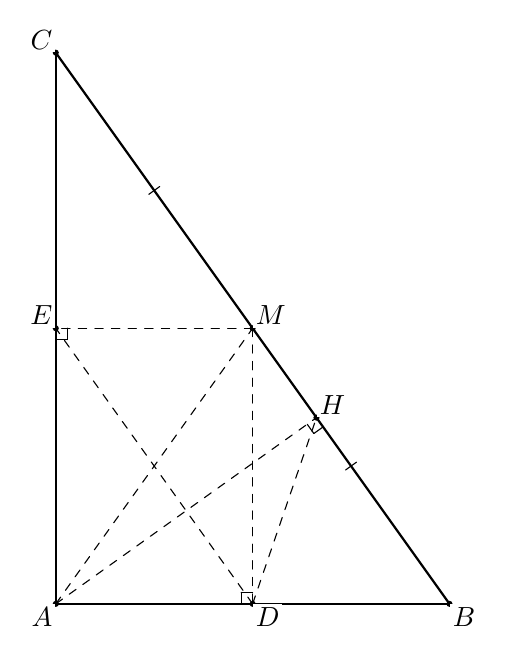
\begin{tikzpicture}[scale=1,line cap=round,line join=round]
\coordinate (p0) at (0,0);
\coordinate (p1) at (5,0);
\coordinate (p2) at (0,7);
\coordinate (p3) at (2.5,3.5);
\coordinate (p4) at (2.5,0);
\coordinate (p5) at (0,3.5);
\coordinate (p6) at (3.3108108,2.3648649);
\draw[thick] (p0) -- (p1);
\draw[thick] (p1) -- (p2);
\draw[thick] (p0) -- (p2);
\draw[dashed] (p3) -- (p4);
\draw[dashed] (p3) -- (p5);
\draw[dashed] (p0) -- (p6);
\draw[dashed] (p0) -- (p3);
\draw[dashed] (p4) -- (p5);
\draw[dashed] (p4) -- (p6);
\draw[dashed] (p6) -- (p3);
\draw[dashed] (p3) -- (p2);
\draw (3.6808327,1.7005948) -- (3.8191673,1.7994052);
\draw (1.1808327,5.2005948) -- (1.3191673,5.2994052);
\draw (2.5,0.1445) -- (2.3555,0.1445);
\draw (2.3555,0.1445) -- (2.3555,0);
\draw (0.1445,3.5) -- (0.1445,3.3555);
\draw (0.1445,3.3555) -- (0,3.3555);
\draw (3.1932263,2.2808759) -- (3.2772152,2.1632915);
\draw (3.2772152,2.1632915) -- (3.3947997,2.2472804);
\fill (p0) circle (1.1pt) node[fill=white,inner sep=1pt,below left] {$A$};
\fill (p1) circle (1.1pt) node[fill=white,inner sep=1pt,below right] {$B$};
\fill (p2) circle (1.1pt) node[fill=white,inner sep=1pt,above left] {$C$};
\fill (p3) circle (1.1pt) node[fill=white,inner sep=1pt,above right] {$M$};
\fill (p4) circle (1.1pt) node[fill=white,inner sep=1pt,below right] {$D$};
\fill (p5) circle (1.1pt) node[fill=white,inner sep=1pt,above left] {$E$};
\fill (p6) circle (1.1pt) node[fill=white,inner sep=1pt,above right] {$H$};
\end{tikzpicture}
\end{document}
